\documentclass[11pt]{article}
\usepackage{graphicx}
\usepackage{amsmath}
\usepackage{siunitx}
\usepackage[super]{nth}
%\usepackage{hyperref}

\title{Investigation on Relationship Between Location of Fretted Note on Guitar Neck and Note Intonation.}
\author{IB Physics Extended Essay}
\begin{document}
    \maketitle
    \tableofcontents

    \begin{flushleft}
    \section{Introduction}
        \subsection{Personal observation}
            Music and sound have always held a special place in my heart, not only as a form of entertainment but also as a means of self-expression and creativity. Since a very young age, I have been fascinated with and have pursued stringed instruments like basses and guitars. Through playing these instruments, I have been able to explore the different components of music and sound, and have developed a keen ear for tone and texture. However, recently I have become increasingly aware of the importance of intonation, which refers to the accuracy of the instrument's pitch across all frets. While playing the guitar, I have noticed that even slight deviations in intonation can have a significant impact on the overall sound quality. This change in intonation often starts around fret 7-8 and above, and most noticeable especially when I play chords high up the neck with a distortion pedal. This is because the higher harmonic frequencies from the distortion will clash with the other notes in the chord when the intonation is not perfect. This will result in a very muffled, discordant sounding chord. This intonation problem has been a topic of debate in many guitar forums online, with a lot of hypotheses on why it happens and discussions on how to set a perfect intonation. Therefore this motivated me to combine it with my love of physics and investigate the principles behind this problem. I want to explore how intonation works, why the note intonation is “off” when you fret a string on high frets, and from there propose solutions to achieve perfect intonation. This investigation is not only significant for my hobby of playing the guitar, but it is also a topic of interest for many musicians and music lovers worldwide. By delving deeper into the science behind the intonation, I hope to not only improve my skills as a guitarist but also contribute to the broader community of music enthusiasts.
        \subsection{Background information}
            \subsubsection*{Basic model of guitar strings and frets}
                The most simple model of an electric guitar basically consists of a piece of steel string anchored at two ends by the bridge saddle and the nut (closer to the fretboard). One end is usually wrapped around a tuning peg to make the string tension adjustable to tune the string to a fixed frequency. This is stretched over a pickup - to capture the string vibrations and turn it into electrical signals - and a fretboard - a long piece of wood with raised metal frets. The fret distances are carefully calculated and accurately placed along the length of the string, so that when the string is pressed down in a fret, the fret itself will act as a stopper and change the length of the vibrating string, thereby changing the vibrating frequency to make other notes in a scale. 
                \begin{figure}[h]
                    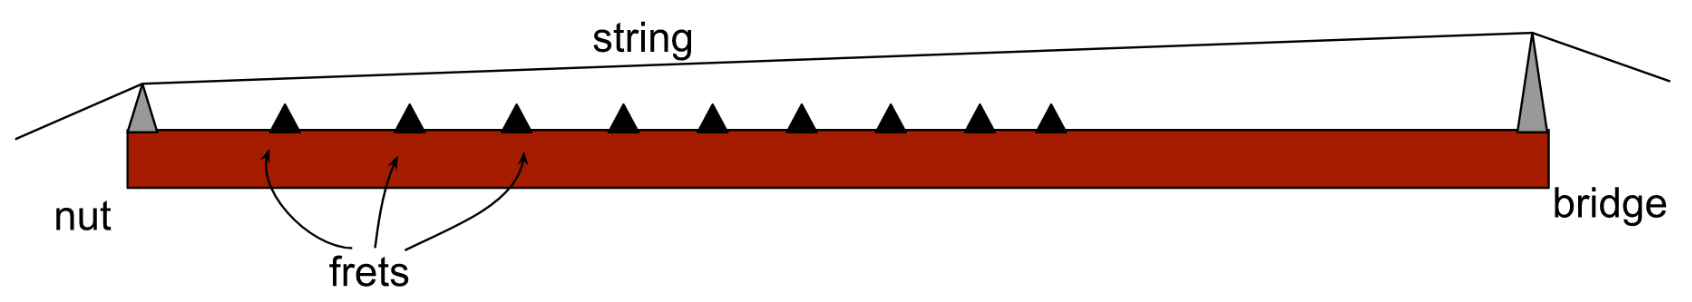
\includegraphics[width=\textwidth]{fig1.png}
                    \caption{A simplified model of the electric guitar I will use. The pickup has been removed.}\label{fig1}
                \end{figure} 
            \subsubsection*{How the guitar string produces sound}
                When the string is plucked, it will create travelling waves on the string that reflect at both ends, creating standing waves. The frequency of the standing waves with the longest wavelength is the fundamental frequency, also called the first harmonic. This is the lowest frequency, and there will usually be other higher harmonics that when combined together create the characteristic timbre of the electric guitar. 
                \begin{figure}[h]
                    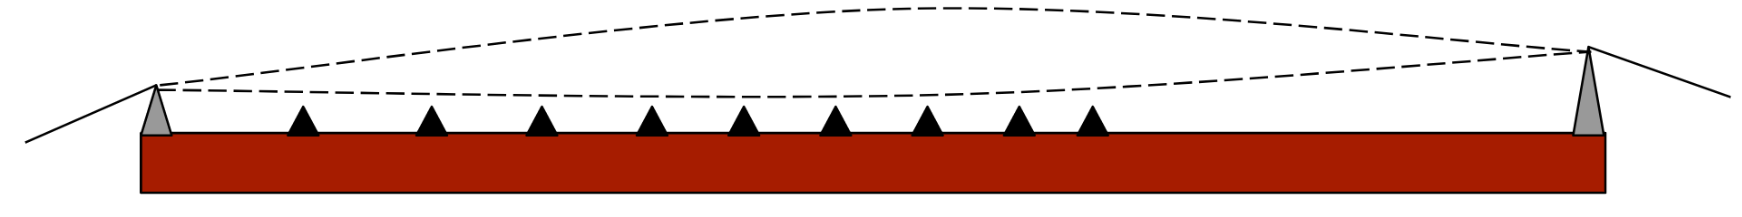
\includegraphics[width=\textwidth]{fig2.png}
                    \caption{The “open” string (not fretted) is plucked and vibrating at its fundamental frequency.}\label{fig2}
                \end{figure} 
            
                The fundamental frequency $f_0$ of a string is determined by this formula
                \begin{equation}\label{eqn1}
                    f_0 = \frac{v}{\lambda}
                \end{equation}
                where $v$ is the speed of the wave on the string and $\lambda$ is the wavelength. 

                From Figure \ref{fig2} we see the wavelength is double the length of the guitar - the “scale length” $l$ . Therefore \begin{equation}\label{eqn2}
                    \lambda = 2l
                \end{equation}
                The speed of the wave $v$ on a stretched string with tension $T$ can be determined by the equation:
                \begin{equation}\label{eqn3}
                    v = \sqrt{\frac{T}{\mu}} 
                \end{equation}
                Where $\mu$ is the linear density of the string (mass of string per unit length)
                Substitute (\ref{eqn2}) and (\ref{eqn3}) into (\ref{eqn1}) we get the expression for the frequency of an open string
                \begin{equation}\label{eqn4}
                    f_0 = \frac{1}{2l}\sqrt{\frac{T}{\mu}}
                \end{equation}

            \subsubsection*{How frets work}
                When the string is pressed down on a fret and plucked, its vibrating length changes which  changes the frequency as well.
                Let's say we press down on fret $n$. The distance from the saddle to the fret then is $l_n$
                
                \begin{figure}[!ht]
                    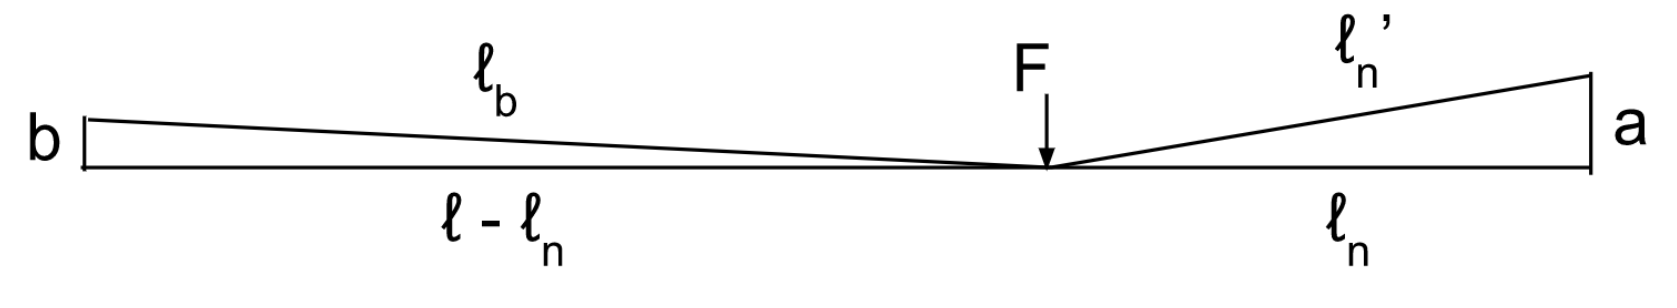
\includegraphics[width=\textwidth]{fig3.png}
                    \caption{A simplified model of the fretted string}\label{fig3}
                \end{figure} 

                Theoretically, the frequency of this note is 
                \begin{equation}\label{eqn5}
                    f_n = \frac{1}{2l_n}\sqrt{\frac{T}{\mu}}
                \end{equation}

                In order to make the frequency match with a specific note in the Western twelve-tone equal temperament (12-TET) system, the scale length needs to be divided into powers of $\sqrt[12]{2}$. To do this luthiers traditionally use a formula to calculate the position of each fret.

                \begin{equation}\label{eqn6}
                    l_n=\frac{l}{2^\frac{n}{12}}
                \end{equation}
                
            \subsubsection*{Cause of intonation issues}
                When pressed down, due to the distance between the nut and the saddle to top of the frets ($b$ and $a$ respectively in Figure \ref{fig3}), the vibrating string length also stretches. The effective vibrating length is now $l_n'$. The fretting force $F$ also causes an increase in tension of the whole string, so the tension now is $T+ \Delta T$. \\
                Therefore, taking into account the fretting action, the frequency now will no longer be the same as the intended frequency $f_n$. This explains why we observe the intonation problem when fretting down on the string. We will call this new frequency $f_n'$
                \begin{equation}\label{eqn7}
                    f'_n= \frac{1}{2l_n'}\sqrt{\frac{T+\Delta T}{\mu}}
                \end{equation}
                
                The intonation deviation is then simply
                \begin{align}
                    \Delta f &= f_n'-f_n \\
                    &= \frac{1}{2\sqrt{\mu}} \left( \frac{\sqrt{T+\Delta T}}{l_n'} - \frac{\sqrt{T}}{l_n} \right)\label{eqn9}
                \end{align}
                
                From Figure \ref{fig3}, using Pythagoras' Theorem for $l_n'$ we get
                \begin{align}
                    l_n' &= \sqrt{l_n^2+a^2} \\
                    &= \sqrt{l_n^2\left(1+\left(\frac{a}{l_n}\right) ^2\right)} \\
                    &= l_n \sqrt{1+\left(\frac{a}{l_n}\right) ^2} \\
                    &= l_n \left(1+\left(\frac{a}{l_n}\right) ^2\right)^{\frac{1}{2}} 
                \end{align}
                Subbing this into (\ref{eqn9}):
                \begin{align}
                    \Delta f &= \frac{1}{2\sqrt{\mu}} \left( \frac{\sqrt{T+\Delta T}}{l_n\sqrt{1+\left(\frac{a}{l_n}\right) ^2}} - \frac{\sqrt{T}}{l_n} \right) \\
                    &= \frac{1}{2l_n\sqrt{\mu}} \left( (T+\Delta T)^{\frac{1}{2}} \left( 1+\left(\frac{a}{l_n}\right) ^2\right)^{-\frac{1}{2}} - \sqrt{T} \right) \\
                    &= \frac{1}{2l_n\sqrt{\mu}} \left( T^{\frac{1}{2}}\left(1+\frac{\Delta T}{T}\right)^{\frac{1}{2}} \left( 1+\left(\frac{a}{l_n}\right) ^2\right)^{-\frac{1}{2}} - \sqrt{T} \right) \\
                    &= \frac{1}{2l_n} \sqrt{\frac{T}{\mu}}\left(\left(1+\frac{\Delta T}{T}\right)^{\frac{1}{2}} \left( 1+\left(\frac{a}{l_n}\right) ^2\right)^{-\frac{1}{2}} - 1 \right)
                \end{align}

                Since $\Delta T$ is much smaller than T, and similarly $a$ is much smaller than $l_n$, we can approximate this to the first order
                \begin{align}
                    \Delta f &\approx \frac{1}{2l_n} \sqrt{\frac{T}{\mu}} \left( \left(1+\frac{\Delta T}{2T}\right) \left( 1- \frac{a^2}{2{l_n}^2} \right) - 1\right) \\
                    &= \frac{1}{2l_n} \sqrt{\frac{T}{\mu}} \left( -\frac{a^2}{2{l_n}^2} + \frac{\Delta T}{2T} - \frac{a^2\Delta T}{4T{l_n}^2}\right) \\
                    &\approx \frac{1}{4l_n} \sqrt{\frac{T}{\mu}} \left( \frac{\Delta T}{T} - \frac{a^2}{{l_n}^2} \right) \label{eqn20}
                \end{align}

            \subsubsection*{Tension of the guitar string}
                A stretched guitar string is under tension $T$. When we press down on it, the whole string stretches accordingly by a small amount $\Delta l$. Assuming there is no friction on the point of contact, the tension in the whole string increases by an amount $\Delta T$
                \begin{equation}
                    \Delta T = \frac{AY\Delta l}{l}\label{eqn21}
                \end{equation} 
                Where $A$ is the cross sectional area of the string, and $Y$ is the Young's modulus of the material.
                The total amount of stretch of the string $\Delta l$ can be calculated from Figure \ref{fig3}. 
                \begin{align}
                    \Delta l &= (l_b + l_n') - l \\
                    &= \sqrt{(l-l_n)^2+b^2} + \sqrt{l_n^2+a^2} - l \\
                    &= (l-l_n)\sqrt{1+\left(\frac{b}{l-l_n}\right)^2} + l_n\sqrt{1+\left(\frac{a}{l_n}\right)^2} - l\\
                    &= (l-l_n)\left(1+\left(\frac{b}{l-l_n}\right)^2\right)^{\frac{1}{2}} + l_n\left(1+\left(\frac{a}{l_n}\right)^2\right)^{\frac{1}{2}} - l
                \end{align}
                Once again, we can approximate this to the first order since both $a$ and $b$ are much smaller than $l_n$ and $l-l_n$. Therefore,
                \begin{align}
                    \Delta l &\approx (l-l_n)\left(1+\frac{b^2}{2(l-l_n)^2}\right)+ l_n\left(1+\frac{a^2}{2l_n^2}\right) - l \\
                    &= (l - l_n) + \frac{b^2}{2(l-l_n)} + l_n + \frac{a^2}{2l_n} - l \\
                    &= \frac{b^2}{2(l-l_n)} + \frac{a^2}{2l_n}
                \end{align}
                Substituting this into (\ref{eqn21}) we get
                \begin{equation}
                    \Delta T = \frac{AY}{2l} \left( \frac{b^2}{l-l_n} + \frac{a^2}{l_n} \right) \label{eqn29}
                \end{equation}
            \subsubsection*{Final expression relating frequency change and position of fret}
                Finally, we can substitute (\ref{eqn29}) into (\ref{eqn20}) to get the expression between the intonation shift $\Delta f$ and the fret position $l_n$
                \begin{align}
                    \Delta f &= \frac{1}{4l_n} \sqrt{\frac{T}{\mu}} \left( \frac{AY}{2Tl} \left( \frac{b^2}{l-l_n} + \frac{a^2}{l_n} \right) - \frac{a^2}{{l_n}^2} \right) \label{eqn30}
                \end{align}
                From (\ref{eqn4}) we get
                \begin{equation*}
                    \sqrt{\frac{T}{\mu}} = 2lf_0
                \end{equation*}
                and 
                \begin{equation*}
                    T = 4\mu l^2{f_0}^2    
                \end{equation*}
                Subbing into (\ref{eqn30})
                \begin{equation}
                    \Delta f = \frac{l f_0}{2l_n} \left( \frac{AY}{8\mu l^3 {f_0}^2} \left( \frac{b^2}{l-l_n} + \frac{a^2}{l_n} \right) - \frac{a^2}{{l_n}^2} \right) \label{eqn31}
                \end{equation}
                

    \section{Experiment}
        From the final expression relating $\Delta f$ and $l_n$, knowing all other constants I can plot the graph for this. $\Delta f$ is the dependent variable, and $l_n$ is the independent variable. It is impossible to linearize the equation, therefore I will have to resort to collecting the data, plotting the graph, then confirming the relationship using a regression method to see how well the data fits the model. 
        The choice of guitar I will use for this experiment is a Fender Stratocaster. This is arguably the most iconic and popular guitar in history, known for its versatility and playability. Therefore I pick this guitar because there is a wealth of information available on it, to make it easier to find data to support my research or to compare my results to other studies. Also due to its popularity, the Stratocaster is a well-known and well-understood instrument. This can make it easier to control variables in my experiment and ensure consistent results.
        The choice of string I will use is a G string from D'Addario's set of Nickel Wound Regular Light Gauge - EXL110-10P that I have at home. I choose the G string because it is the thickest string in the set that is a plain unwound string. This is because the thicker string will make the effects of the intonation shift more noticeable. %cite this
        \subsection{Determining the constants}
            From the equation (\ref{eqn31}), the constants I need to determine are $f_0$, $\mu$, $A$, $Y$, $a$, $b$ and $l$. 
            \begin{itemize}
                \item $l$ is the scale length of the guitar. For a Fender Stratocaster, it is 25.5 inches (64.77cm). I round this up to 64.8cm (3s.f). From this information, I can adjust the bridge saddle position so that the scale length matches 64.8cm (0.648 m)
                \item Initial frequency $f_0$ can be measured directly in the experiment. Frequency we aim for is the frequency of G string on the guitar, $G_3$ at 196 Hz
                \item Young's modulus $Y$ is dependent on the specifications of the string material. The string I use follows the ATSM-A228 standard, and the accepted literature value of $Y$ is \SI{210}{\giga\pascal} (\SI{2.10e11}{\pascal})
                \item $A$ - the cross-sectional area of the string. This can be calculated based on the diameter of the string. For this string set, the G string gauge is 17-gauge, which is equivalent to a diameter of 0.017 inches (0.4318 mm). Using the formula for area of a circle from diameter:
                \begin{align*}
                    A &= \frac{\pi d^2}{4} \\
                    &= \SI{1.464e-7}{\meter}
                \end{align*}
                \item $\mu$, the linear density of the string, is determined as \\
                \begin{equation*}
                    \mu = \frac{m}{l} = \frac{\rho V}{l} = \frac{\rho l A}{l} = \rho A
                \end{equation*}
                where $m$ is the mass of the vibrating string section, $V$ is its volume, and $\rho$ is the volumetric density of the material. According to ATSM-A228 standards, $\rho = \SI{7.80e3}{\kg.m^{-3}}$.
                \begin{equation*}
                    \mu = \num{7.80e3} \cdot \num{1.46e-7} = \SI{1.14e-3}{kg.m^{-1}}
                \end{equation*}
                \item $a$ and $b$: it is very hard to measure these directly, as they are distance from the nut and saddle to the top of the fret, not the height itself. Therefore I can only set up the guitar indirectly according to recommended values and calculate them afterwards. I follow the instructions by Stewmac, and take the average value of the action (distance between string and top of fret) for the \nth{1} fret to be 0.016" (0.406mm) and \nth{12} fret to be 0.070" (1.78mm). I change the adjustable saddle height and file down/shim up the nut height to match these values. From there I can calculate the values of $a$ and $b$: \\
                \begin{figure}[ht]
                    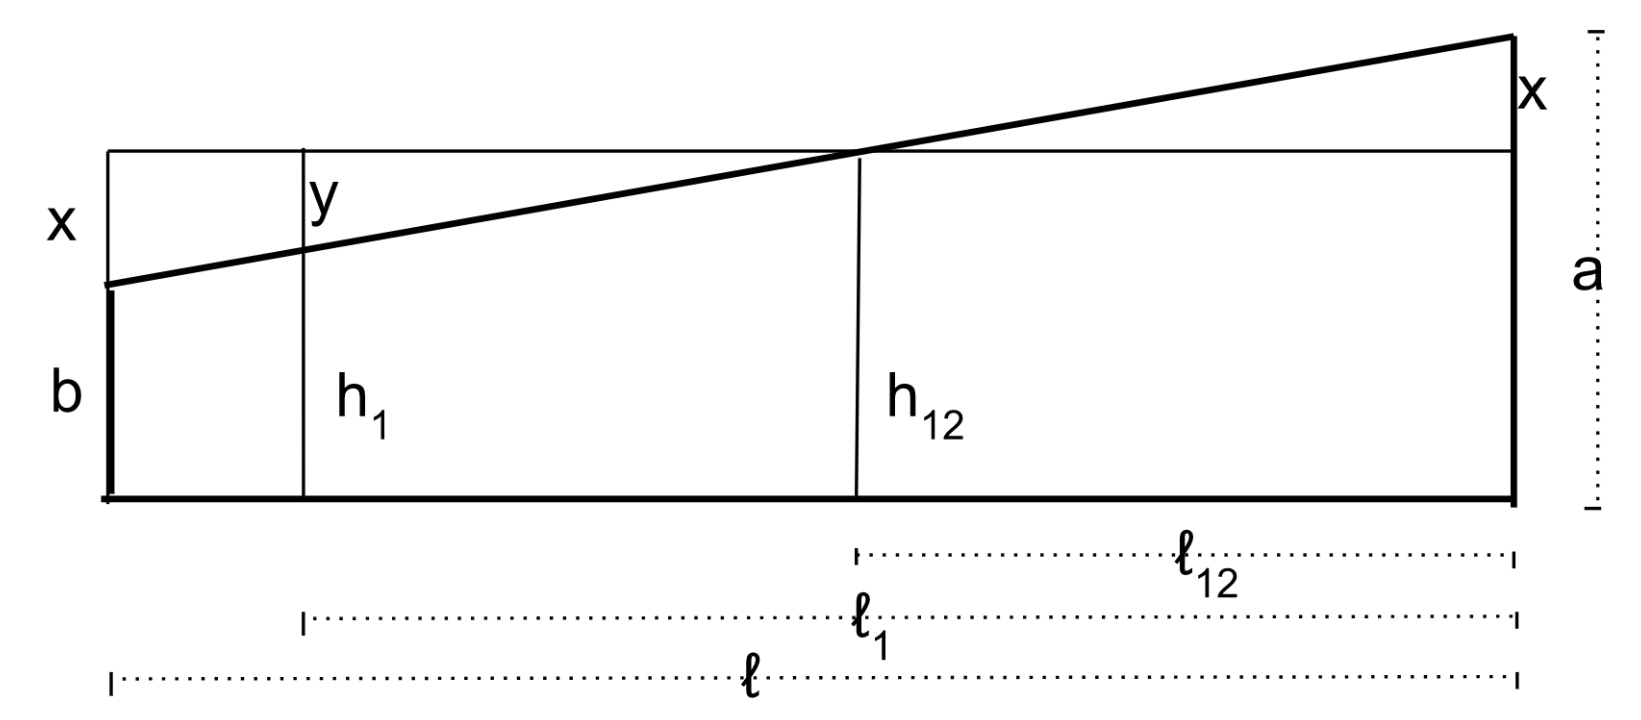
\includegraphics[width = \textwidth]{fig4.png}
                    \caption{Diagram to calculate values of $a$ and $b$} \label{fig4}
                \end{figure}
                Since fret \nth{12} is exactly in the middle of l ($l_{12} = \frac{l}{2} = \frac{.648}{2} = .324$ m) we get a pair of congruent triangles as highlighted. Therefore:
                \begin{align*}
                    a &= h_{12} + x \\
                    b &= h_{12} - x
                \end{align*}
                From the luthier formula (\ref{eqn6}) we get
                \begin{align*}
                    l_1 &= \frac{l}{2^{\frac{1}{12}}} \\
                        &= \frac{.648}{2^{\frac{1}{12}}} \\
                        &= \SI{.612}{\meter}
                \end{align*}
                and we also get the ratio in Figure \ref{fig4}
                \begin{align*}
                    \frac{x}{y} &= \frac{l-l_{12}}{l_1-l_{12}} \\
                    x &= y\frac{l-l_{12}}{l_1-l_{12}} \\
                    &= (h_{12}-h_1)\frac{l-l_{12}}{l_1-l_{12}} \\
                    &= (1.78-.406) \cdot 10^{-3} \cdot \frac{.648-.324}{.612-.324} \\
                    &= \SI{1.55e-3}{\meter}
                \end{align*}
                Therefore
                \begin{align*}
                    a &= 1.78 + 1.55 = \SI{3.33e-3}{\meter} \\
                    b &= 1.78 - 1.55 = \SI{1.30e-4}{\meter}
                \end{align*}    
            \end{itemize}
        \subsection{Apparatus}
            \begin{itemize}
                \item 1 Fender Stratocaster style guitar
                \item 1 17-gauge plain unwound steel G string
                \item 1 guitar capo 
                \item 1 guitar pick
            \end{itemize}
        \subsection{Process}
            \begin{enumerate}
                \item Setting up the guitar. I used the instructions by Stewmac %cite
                \item Connect the guitar to frequency measuring software. I used my audio interface to connect the guitar to my laptop, and the software I used is Visual Analyzer 2020. I chose this because it supports FFT (Fast Fourier Transform) in real-time and can be configured to provide results with high accuracy. 
                \item Measure $f_0$ by plucking the string with no capo on.
                \item Pluck it 5 times with the pick, changing the plucking position each time, from above the neck pickup, to between neck and middle pickups, above middle, between middle and bridge, and above bridge pickup. Record the peak frequency (highest dB) for each pick. \label{enum4}
                \item Put capo on \nth{7} fret and repeat step \ref{enum4}. \label{enum5}
                \item Repeat step \ref{enum5} from fret 7 up to fret 16. I cannot go higher than this because it is impossible to put the capo.
            \end{enumerate}
            \begin{figure}
                \includegraphics[w = textwidth]{name}
            \end{figure}
        
    \end{flushleft}

\end{document}